%%{ DOC HEAD

\pdfoutput=1
\documentclass[a4paper,12pt,titlepage, twoside]{article}
\usepackage[english]{babel}
\usepackage[utf8]{inputenc}
\usepackage{amssymb,amsmath}
\usepackage{algorithm,algpseudocode}
\usepackage[title,titletoc]{appendix}
\usepackage{latexsym}
\usepackage{a4wide}
\usepackage{color}
\usepackage{indentfirst}
\usepackage{graphicx}       %%% graphics for dvips
\usepackage{fancyhdr}
\usepackage{longtable}
\usepackage{pifont}
\usepackage{makeidx}
\usepackage{lastpage}
\usepackage{multirow}
\usepackage{dcolumn}
\usepackage{epstopdf}
\usepackage{url}
\usepackage{listings}
\usepackage{caption}
\usepackage{subcaption}
\usepackage{relsize}
\usepackage{pdfpages}
\usepackage{url}

%%{ custom macros

\newcommand{\unit}[2]{$#1~\ensuremath{\mathrm{#2}}$}
\newcommand{\strong}[1]{\textbf{#1}}
\newcommand{\coord}[1]{\textbf{#1}}
\newcommand{\norm}[1]{\left\lvert#1\right\rvert}
\newcommand{\m}[1]{\ensuremath{\mathbf{#1}}}
\newcommand\numberthis{\addtocounter{equation}{1}\tag{\theequation}}
\newcommand{\corrected}[1]{{\color{black} {#1}}}
\newcommand{\updated}[1]{{\color{black} {#1}}}

%%}

\newcommand{\Author}{Ing. Tomáš Báča}
\newcommand{\Supervisor}{Ing. Martin Saska, Dr. rer. nat.}
\newcommand{\Title}{Distributed Sensing with Group of Unmanned Aerial Vehicles}
\newcommand{\DocName}{Thesis}
\newcommand{\Keywords}{mobile robotics}
\newcommand{\Date}{1/1/2019}
\newcommand{\DOCVersion}{0.1}

\def\clinks{false}

\lstset{breaklines=true,captionpos=b,frame=single,language=sh,float=h}
\lstloadlanguages{sh,c}
\def\lstlistingname{Listing}%{Výpis}
\def\lstlistlistingname{Listings}%{Seznam výpisů}

% European layout (no extra space after `.')
\frenchspacing

% no indent, free space between paragraphs
\setlength{\parindent}{1cm}
\setlength{\parskip}{1ex plus 0.5ex minus 0.2ex}

\pagestyle{fancy}
\setlength{\headheight}{18pt}
\renewcommand{\footrulewidth}{0.4pt}

%\lfoot{ČVUT FEL, Katedra Kybernetiky, Gerstner Laboratory}
\cfoot{}
%\rfoot{\thepage$/$\pageref{LastPage}}

\fancypagestyle{plain}

\fancyhead[R]{}

\begin{document}

%%}

%%{ INTRODUCTION

\section{Introduction}

%%}

%%{ IONIZING RADIATION IMAGING

\section{Ionizing radiation imaging}

%%{ TIMEPIX DETECTOR

\subsection{Timepix detector}

%%}

\clearpage

%%{ INTERACTION OF IONIZING INTERACTION WITH MATTER

\section{Interaction of ionizing radiation with matter}

\subsection{Ionizing radiation}

\subsection{Photo-electric effect}

Photo-electric effect (Einstein, Nobel prize, 1905) describes a total absorption of a photon by an electron.
When the electron is absorbed, the energy of the photon is completely consumed.
A portion of the energy is responsible for releasing the electron from the atomic orbital, the rest is converted to the electron's kinetic energy.

%%{ COMPTON SCATTERING

\subsection{Compton scattering}

Compton scattering occurs when a photon transfers a portion of its energy to an electron.
During this interaction, the photon is deflected from its original path by the radial angle $\theta$ and azimuthal angle $\phi$.

%%{ DIFFERENTIAL CROSS SECTION

In a classical mechanics, the properties of non-elastic scattering of a particle from an object (scattering center) is described by a differential cross section.

\subsubsection{Differential cross section}

Considering a single particle on an incident trajectory with the scattering object.
The displacement $b$ of the particle from the path to the scattering center is called the impact parameter, the radial angle of scattering is denoted as $\theta$.
Various types of reactions have distinct relation between $b$ and $\theta$.

The total area of the impact parameter is the impact cross section $\sigma$, which can be obtained by integrating the impact parameter $b$ over all possible azimuthal angles $\phi$:
\begin{equation}
  \sigma\left(b\right) = \int_\Phi b\left(\phi\right)\,d\phi.
\end{equation}
In a case where the scattering does not influence $\phi$ (axially symmetrical case), the impact cross section takes following form
\begin{equation}
  \sigma\left(b\right) = \int_\Phi b\,d\phi = \frac{b^{2}}{2}\,2\pi = \pi\,b^2.
\end{equation}
Such relaxation is viable for Compton scattering, since the scattering bodies are spherically symmetrical objects.
The differential of the impact cross section is
\begin{equation}
  d\sigma\left(b\right) = \frac{\partial \sigma}{\partial b}\,db = 2\pi\,b\,db.
\end{equation}

\begin{equation}
  \Omega\left(r, \Theta\right) = \int_0^\Theta 2\pi r\,\cos\theta\,r\,d\theta = \left[-2\pi r^2\,\sin\theta\right]_0^\Theta = 2\pi r^2 - 2\pi r^2\cos\Theta
\end{equation}
The differential of the area is
\begin{equation}
  d\Omega\left(\theta\right) = \frac{\partial \Omega}{\partial r}\,dr + \frac{\partial \Omega}{\partial \theta}\,d\theta = -4\pi r\,\cos\theta\,dr + 4\pi r\,dr + 2\pi r^2\sin\theta\,d\theta
\end{equation}
In the case of a unit sphere, the differential of the area becomes
\begin{equation}
  d\Omega(\theta) = 2\pi r^2\sin\theta\,d\theta.
\end{equation}

\begin{figure}[ht]
  \centering
  \begin{subfigure}{0.49\textwidth}
    \centering
    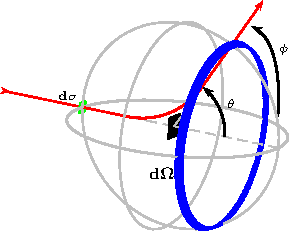
\includegraphics[width=0.8\textwidth]{./fig/compton_scattering_illustration_1.pdf}
    \caption{Showcase of solid angle $d\Omega$ and the differential size of the impact plane $d\sigma$ for $\theta=$~\unit{60}{deg}.}
    \label{fig:differential_cross_section_1}
  \end{subfigure}
  \begin{subfigure}{0.49\textwidth}
    \centering
    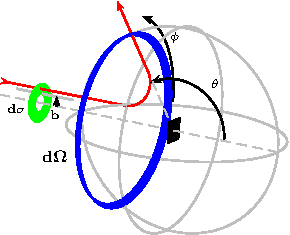
\includegraphics[width=0.8\textwidth]{./fig/compton_scattering_illustration_2.pdf}
    \caption{Showcase of solid angle $d\Omega$ and the differential size of the impact plane $d\sigma$ for $\theta=$~\unit{120}{deg}.}
    \label{fig:differential_cross_section_2}
  \end{subfigure}
  \caption{Illustration of the differential cross section for two possible values of $\theta$. The solid angle $d\Omega$ is integrated of all values of $\phi$ since the azimuthal angle $\phi$ is not changed by the scattering process.}
  \label{fig:differential_cross_section}
\end{figure}

%%}

The ratio $E_r$ of the energy of incoming ($E_{0}$) and scattered ($E_{s}$) particles was observed and described by Compton as
\begin{equation}
  E_r\left(\theta, E_0\right) = \frac{E_s\left(\theta, E_0\right)}{E_{0}} = \frac{1}{1 + \frac{E_0}{m_ec^2}\left(1 - \cos\theta\right)},
\end{equation}
where $\theta \in \left[-\pi, \pi\right)$ is the radial angle at which the photons are scattered, $E_0, E_s$ $\left[\mathrm{J}\right]$ are the energies of the incoming and scattered photons, \unit{m_e \approx 9.10 \times 10^{-31}}{kg} is the invariant mass of the electron, \unit{c \approx 2.99 \times 10^{8}}{ms^{-1}} is the speed of light in vacuum.

The Klein-Nishina formula \cite{leo2012techniques} describes the differential cross section of the incident and scattered beam as
\begin{equation}
  \frac{d\sigma}{d\Omega}\left(\theta\right) = \frac{1}{2}\,r_{e}^2\,E_r\left(\theta\right)^2\left(E_r\left(\theta\right) + \frac{1}{E_r\left(\theta\right)} - \sin^2\theta\right),
\end{equation}
where \unit{r_e \approx 2.81 \times 10^{-15}}{m} is the classical electron radius.

% The intensity of the scattered beam \unit{N_s}{\left[s^{-1}\right]} is calculated for a small finite solid angle \unit{\Delta \theta}{\left[sr\right]} as
% \begin{equation}
%   N_s = N_o\,\frac{d\sigma}{d\Omega}\left(\theta\right)\,n_e\,t\,\Delta\theta,
% \end{equation}
% where \unit{N_0}{\left[s^{-1}\right]} is the intensity of the incoming beam, \unit{n_e}{\left[m^{-3}\right]} is the electron density of the scattering material and \unit{t}{\left[m\right]} is the effective thickness of the scattering material.

\begin{equation}
  \sigma = \oint_{4\pi} \frac{d\sigma}{d\Omega}\,d\Omega = \int_0^{2\pi} \int_0^{\pi} \frac{d\sigma}{d\Omega}\sin\theta\,d\theta\,d\phi,
\end{equation}

Photon attenuation, i.e., the decrease of the intensity $d\Phi$ of an incident beam with original flux $\Phi \left[\mathrm{s}^{-1}\right]$ is described as
\begin{equation}
  \frac{d\Phi}{dz} = -n\sigma\Phi
\end{equation}
where $dz$ is the thickness of the blocking material, \unit{n_e}{\left[m^{-3}\right]} is the electron density of the scattering material and $\sigma \left[\mathrm{m}^{2}\right]$ is the total cross section of the interaction.
By solving the differential equation, we obtain a relationship between the initial flux $\Phi$ and the remaining flux $\Phi_{out}$ behind the object with the thickness $z$:
\begin{equation}
  \Phi_{out} = \Phi e^{-n\sigma z}.
\end{equation}
This the probability of a Compton scattering $\mathrm{P}\left(c\right)$ is modeled as
\begin{equation}
  \mathrm{P}\left(c\right) = 1 - e^{-n\sigma z}.
\end{equation}

\begin{equation}
  \mathrm{P}\left(\theta \mid c\right) = \frac{\int_0^\pi \frac{d\sigma}{d\Omega}\,\sin \theta\,d\phi}{\sigma}
\end{equation}

\begin{equation}
  \mathrm{P}\left(c \mid \theta\right) = \mathrm{P}\left(\theta \mid c\right) \mathrm{P}\left(c\right) = \left(1 - e^{-n\sigma z}\right) \frac{\int_0^\pi \frac{d\sigma}{d\Omega}\,\sin \theta\,d\phi}{\sigma}
\end{equation}

\begin{figure}[ht]
  \centering
  \begin{subfigure}{0.32\textwidth}
    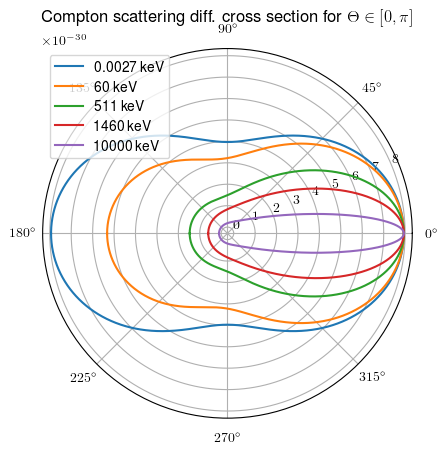
\includegraphics[width=1.0\textwidth]{./fig/klein_nishina_1.png}
    \caption{Plots of the differential $d\sigma/d\Omega$ cross section for various photon energies.}
    \label{fig:klein_1}
  \end{subfigure}
  \begin{subfigure}{0.32\textwidth}
    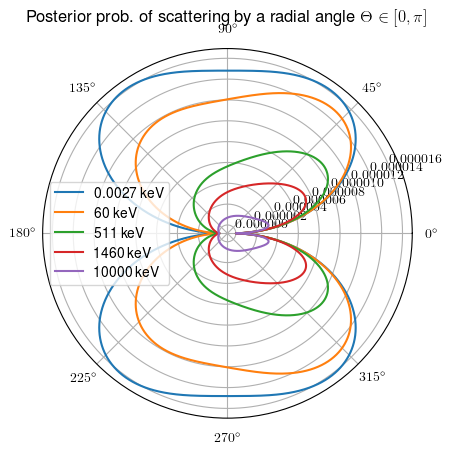
\includegraphics[width=1.0\textwidth]{./fig/klein_nishina_2.png}
    \caption{Plots of posterior probability $\mathrm{P}\left(E_0 \mid \theta\right)$, integrated over azimuthal angle $\phi$.}
    \label{fig:klein_2}
  \end{subfigure}
  \begin{subfigure}{0.32\textwidth}
    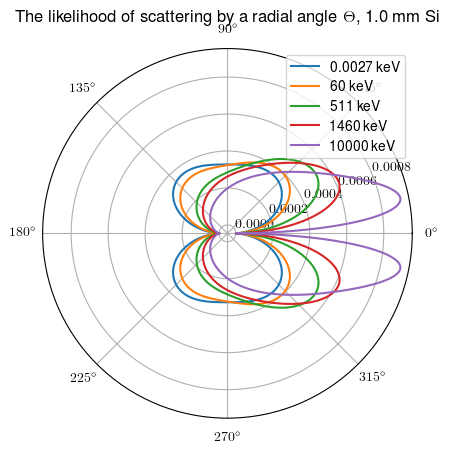
\includegraphics[width=1.0\textwidth]{./fig/klein_nishina_3.png}
    \caption{Plots of likelihood probability $\mathrm{P}\left(\theta \mid E_0\right)$, integrated over azimuthal angle $\phi$.}
    \label{fig:klein_3}
  \end{subfigure}
  \caption{Plots of the Klein-Nishina differential cross section (\ref{fig:klein_1}), the cross section normalized by the total cross section (\ref{fig:klein_2}) and the resulting probability distribution (\ref{fig:klein_3}) invariant on the radial angle $\phi$.}
  \label{fig:klein_nishina}
\end{figure}

%%}

%%{ GAMMA-RAY CAMERA

\subsection{Compton $\gamma$-ray camera}

%%}

%%}

%%}

%%{ RADIATION SOURCE ESTIMATION

\section{Radiation source state estimation}

%%}

%%{ DISTRIBUTED SENSING USING MULTIPLE UAVS

\section{Distributed sensing using multiple UAVs}

%%}

%%{ AUTONOMOUS TRACKING OF A MOVING RADIATION SOURCE

\section{Autonomous tracking of a moving radiation source}

\subsection{Predicting target motion}

%%}

%%{ CONCLUSIONS

\section{Conclusions}

%%}

%%{ DOC BOTTOM

%%{ REFERENCES

\clearpage
\bibliography{main}{}
\cleardoublepage
\bibliographystyle{IEEEtran}
\clearpage

%%}

%%{ APENDICES

% \appendices
% \lhead{\emph{APPENDIX \leftmark}}
% \cleardoublepage

%%}

\end{document}

%%}
